\documentclass{article}
\usepackage{amsmath}
\usepackage{hyperref}
\usepackage{graphicx}
\usepackage{float}
\usepackage[a4paper, margin=1in]{geometry}
\begin{document}

% ROS 2 Robotics Training Module: Navigation and Localization with RTAB-Map

% Introduction

\section*{Modul Pelatihan Teaching Factory Programming: Navigasi dan Lokalisasi dengan RTAB-Map}
Program pelatihan ini dirancang untuk mahasiswa yang sudah memiliki pengetahuan dasar tentang ROS2.
Fokus pelatihan adalah pada navigasi, lokalisasi, navigasi waypoint, dan pengendalian misi menggunakan state machine.
Pelatihan ini menggunakan simulasi TurtleBot dan RTAB-Map.

% Module 1
\section{Modul 1: Setup \& Installasi}

\subsection{Konfigurasi Environment}
\begin{itemize}
  \item Install ROS 2 Humble
        lakukan installasi menggunakan \href{https://docs.ros.org/en/humble/Installation/Ubuntu-Install-Debs.html}{\textbf{panduan instalasi Debian}}
  \item Install TurtleBot3 packages menggunakan \href{https://emanual.robotis.com/docs/en/platform/turtlebot3/quick-start/#installing-turtlebot3-packages}{\textbf{panduan instalasi TurtleBot3}}
  \item Install Gazebo dengan \texttt{sudo apt install ros-humble-desktop}
  \item Install RViz2 dengan \texttt{sudo apt install ros-humble-rviz2}
  \item Install RTAB-Map dengan \texttt{sudo apt install ros-humble-rtabmap-ros}
  \item Install Navigation2 dengan \texttt{sudo apt install ros-humble-navigation2 ros-humble-nav2-bringup}
\end{itemize}

\subsection{Menjalankan Simulasi}
Setelah semua paket terinstal, jalankan simulasi TurtleBot3 Waffle Pi di Gazebo dengan environment \texttt{house}:
\begin{verbatim}
export TURTLEBOT3_MODEL=waffle_pi
ros2 launch turtlebot3_gazebo turtlebot3_house.launch.py
\end{verbatim}

\subsection{Teleoperation}
Buka terminal lain untuk menjalankan teleop:
\begin{verbatim}
ros2 run turtlebot3_teleop teleop_keyboard
\end{verbatim}

\subsection{RViz2}
Buka RViz2 untuk melihat topik yang dipublish dan TF yang dimiliki robot:
\begin{verbatim}
rviz2
\end{verbatim}
Atur Fixed Frame ke \texttt{odom}.
Tambahkan display untuk \texttt{LaserScan}, dan \texttt{TF}.
Sehingga akan muncul tampilan seperti berikut:
\begin{figure}[H]
  \centering
  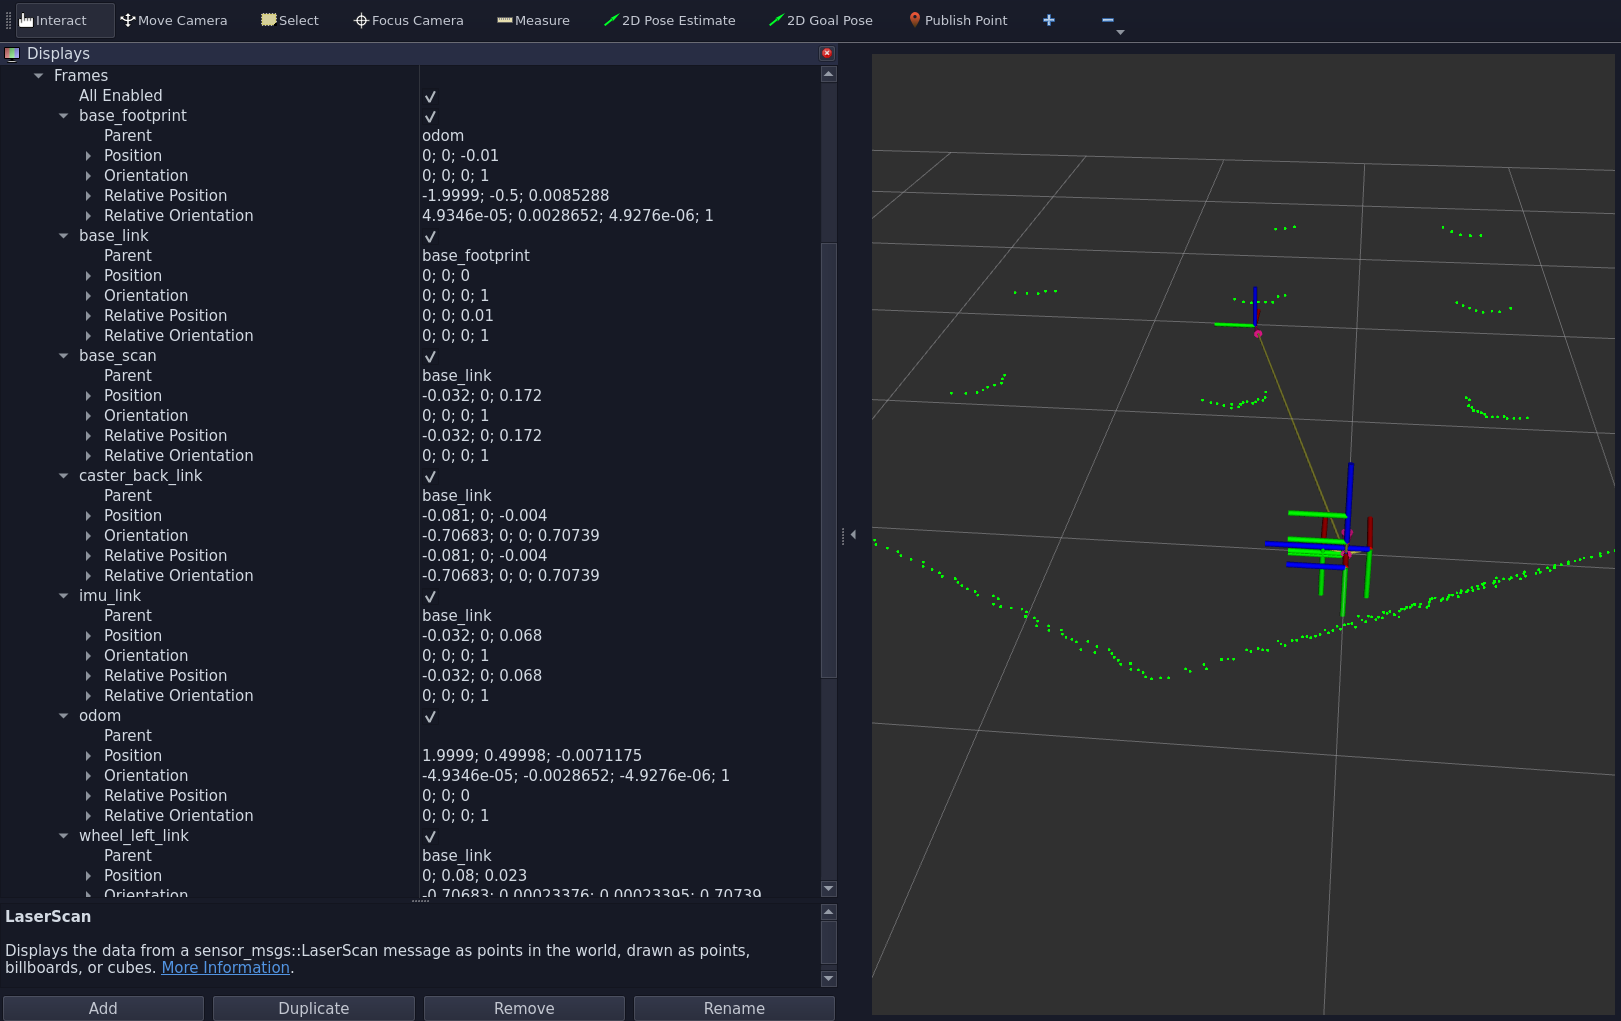
\includegraphics[width=1\textwidth]{rviz2.png}
  \caption{Contoh tampilan RViz2}
\end{figure}

Pada sidebar ditunjukkan TF yang dimiliki robot:
\begin{itemize}
  \item \texttt{odom}: frame odometri, bergerak relatif terhadap \texttt{base\_link}
  \item \texttt{base\_footprint}: frame footprint robot (sejajar dengan ground plane 2D)
  \item \texttt{base\_link}: frame utama robot (dapat mengalami translasi dan orientasi)
  \item \texttt{caster\_back\_link}: frame caster back (free wheel)
  \item \texttt{imu\_link}: frame IMU
  \item \texttt{base\_scan}: frame laser scan
  \item \texttt{wheel\_left\_link}: frame roda kiri
  \item \texttt{wheel\_right\_link}: frame roda kanan
  \item \texttt{camera\_link}: frame dasar kamera (body), menunjukkan posisi fisik kamera pada robot. Orientasi mengikuti konvensi ROS, yaitu $x$ ke depan, $y$ ke kiri, dan $z$ ke atas.
  \item \texttt{camera\_rgb\_frame}: frame kamera RGB (sensor), digunakan sebagai acuan untuk data gambar. Orientasinya sama dengan \texttt{camera\_link}.
  \item \texttt{camera\_rgb\_optical\_frame}: frame kamera dengan konvensi optik. Orientasi mengikuti standar OpenCV, yaitu $z$ ke depan, $x$ ke kanan, dan $y$ ke bawah.
\end{itemize}
Semua TF tersebut terhubung dalam sebuah pohon (tree) yang dapat dilihat pada tab \texttt{TF} di RViz2. atau dengan perintah:
\begin{verbatim}
ros2 run tf2_tools view_frames.py
\end{verbatim}
Perintah ini akan menghasilkan file \texttt{frames.pdf} yang menunjukkan struktur pohon TF sebagai berikut:
\begin{figure}[H]
  \centering
  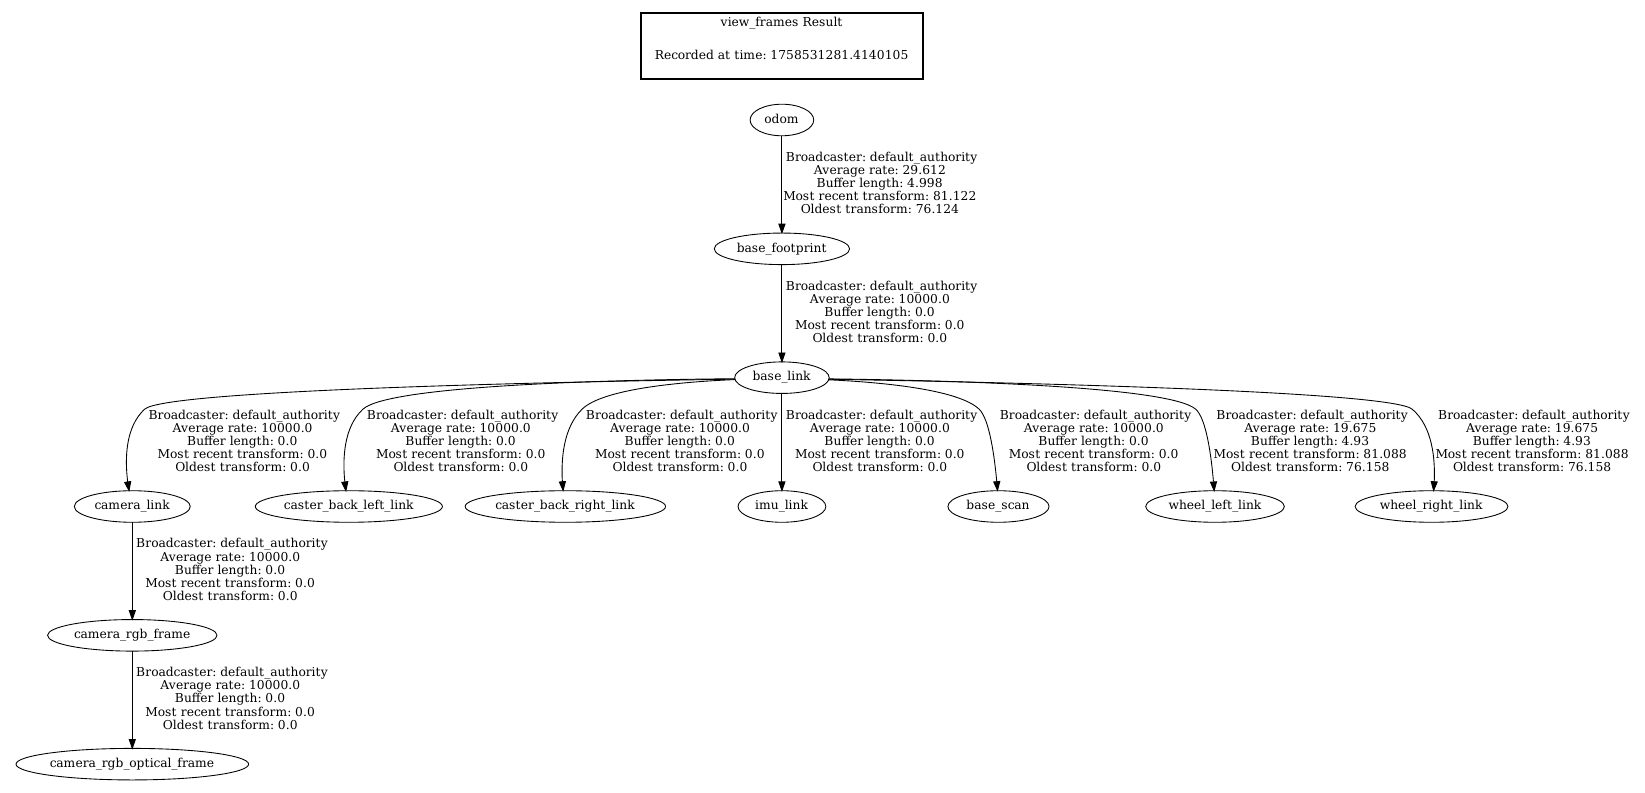
\includegraphics[width=1\textwidth]{tf_tree.png}
  \caption{Contoh TF Tree}
\end{figure}


% Module 2
\section{Modul 2: Mapping dengan RTAB-Map}
\textbf{Objectives:}

\subsection{SLAM dan RTAB-Map}
SLAM (Simultaneous Localization and Mapping) adalah proses di mana robot membangun peta lingkungan sambil menentukan posisinya di dalam peta tersebut. Pada dasarnya, SLAM dibagi menjadi dua yaitu map based SLAM dan graph based SLAM. Perbedaan paling mendasar adalah pada bagian lokalisasinya. Pada map based SLAM, lokalisasi dilakukan dengan melakukan registrasi data sensor ke map yang telah dibangun sebelumnya. Sedangkan pada graph based SLAM, lokalisasi dilakukan dengan registrasi sensor ke setiap graph yang dibangun sebelumnya. 
\par    
RTAB-Map (Real-Time Appearance-Based Mapping) adalah sebuah algoritma graph based SLAM yang menggunakan data visual (gambar) dan data jarak (misalnya dari LIDAR atau depth camera) untuk membangun peta 3D dari lingkungan sekitar. RTAB-Map dapat digunakan untuk berbagai aplikasi robotika, termasuk navigasi, inspeksi, dan pemetaan lingkungan. Untuk memperjelas bagaimana cara kerja Graph Based SLAM, silahkan simak video berikut: \href{https://youtu.be/saVZtgPyyJQ?si=qHGGJnJUz-iB19UF}{\textbf{Graph Based SLAM Explanation}}. 

\subsection{RTAB-Map}
Kunci dari Graph Based SLAM adalah deteksi loop closure. Di RTAB-Map, deteksi loop closure menggunakan kamera. Algoritma dasar yang perlu dipelajari untuk mencari loop closure menggunakan kamera adalah Image Registration. Image Registration adalah proses mencocokkan dua gambar yang diambil dari sudut pandang yang berbeda untuk menemukan transformasi geometris antara keduanya. Contoh contoh algoritma yang sering dipakai adalah GFTT, FAST, BRIEF, ORB, SIFT, dan lain lain.        
\newline
\textbf{RTAB-Map bukanlah Ready to Use SLAM, perlu dilakukan penyesuaian pada robot yang akan digunakan!}

\subsection{Penyesuaian RTAB-Map}
\subsubsection{Penyesuaian Sensor}
  Di RTAB-Map, bisa menggunakan beberapa sensor, cara setting nya lewat parameter:
  \begin{itemize}
    \item \textbf{subscribe\_depth}: Untuk kamera depth seperti realsense 
    \item \textbf{subscribe\_scan}: Untuk LIDAR 2d 
    \item \textbf{subscribe\_scan\_cloud}: Untuk LIDAR 3d
    \item \textbf{subscribe\_rgbd}: Untuk kamera RGBD seperti Kinect
    \item \textbf{subscribe\_stereo}: Untuk kamera stereo seperti Zed
    \item \textbf{subscribe\_odom}: Untuk odometri hardware atau sumber odometry lainnya
  \end{itemize}
  Jika sistem robot tidak memiliki source odometry, odometry bisa dihitung dari visual odometry atau icp odometry bawaan RTAB-Map. Untuk menggunakannya bisa menajalankan node lain yaitu \texttt{rgbd\_odometry} atau \textit{icp\_odometry}. 

\subsubsection{Penyesuaian Loop Closure Detection}
Ada beberapa hal penting yang perlu diperhatikan dalam penyesuaian loop closure detection:
\begin{itemize}
  \item \textbf{Kp/DetectorStrategy}: Memilih algoritma image matching yang sesuai dengan kondisi lingkungan dan jenis kamera yang digunakan. 
  \item \textbf{Kp/MaxFeatures}: Berapa banyak maksimal fitur (words) yang bisa disimpan dalam database. Perhatikan juga setiap algoritma akan menghasilkan jumlah fitur yang berbeda beda.
  \item \textbf{Vis/MinInliers}: Hasil dari scan matching juga berupa inliers yang telah diperoleh dari RANSAC. Semakin besar nilai inliers, semakin baik hasil scan matching. Namun, jika terlalu besar, bisa jadi tidak ada loop closure yang terdeteksi. 
\end{itemize}

\subsubsection{Penyesuaian Graph Optimization}
Graph optimization adalah proses memperbaiki posisi node pada graph berdasarkan loop closure yang terdeteksi. Ada beberapa parameter penting yang perlu diperhatikan:
\begin{itemize}
  \item \textbf{Reg/Strategy}: Memilih mau menggunakan sensor apa untuk menghitung constraint per node pada graphnya. Bisa menggunakan icp atau visual atau gabungan keduanya. ICP dari LIDAR sedangkan visual dari kamera. 
  \item \textbf{Optimizer/Strategy}: Memilih algoritma optimizer yang diinginkan (default GTSAM).
  \item \textbf{Optimizer/Iterations}: Semakin besar maka semakin lama iterasi optimasinya, hasilnya belum tentu lebih baik. Gunakan default saja jika tidak ada masalah.
  \item \textbf{RGBD/OptimizeMaxError}: Gerbang terakhir untuk optimasi, Jika hasil error nya terlalu besar maka loop closure akan di-reject dan graph tidak akan dioptimasi. 
  \item \textbf{RGBD/OptimizeFromGraphEnd}: Ketika loop closure diterima, ada dua pendekatan optimasi, optimasi seluruh graph atau hanya dari node terakhir. Jika optimiasi dari seluruh graph, pasti akan membuat map atau estimasi pose robot loncat.
\end{itemize}

\subsubsection{Parameter Penting Lainnya}
\begin{itemize}
  \item \textbf{Mem/IncrementalMemory}: Dipastikan false, agar database dalam keadaan frozen saat pertama kali dihidupkan. Intinya, keadaan default adalah keadaan lokalisasi, bukan mapping. Jika ingin mapping, harus diaktifkan dengan service.
  \item \textbf{Mem/STMSize}: Berapa banyak node terakhir yang akan disimpan di Short Term Memory (STM). Node-node ini akan dibandingkan dengan node baru untuk mencari loop closure. Jika robot bergerak cepat, maka STM size harus lebih besar.
  \item \textbf{Mem/NotLinkedNodesKept}: Berapa banyak node yang tidak terhubung dengan loop closure yang akan disimpan di memori. Setting ini ke True agar databse tidak crash. 
  \item \textbf{RGBD/NeighborLinkRefining}: Jika TF sensor sudah dipastikan bagus, maka parameter ini bisa diset True. Jika kurang percaya dengan hasil sensor, dan ingin lebih percaya dengan odometry, maka bisa diset False.
\end{itemize}

\subsubsection{Grid Map}
Grid hasil dari RTAB-Map berupa occupancy grid. Hasil dari occupancy grid ini tidak penting untuk lokalisasi karena RTAB-Map merupakan graph based SLAM. Biasanya, grid map ini digunakan untuk navigasi yang nantinya berupa global costmap. Ada beberapa parameter penting yang perlu diperhatikan:
\begin{itemize}
  \item \textbf{Grid/Sensor}: Jenis sensor yang digunakan untuk membuat grid. Bisa menggunakan laser scan, depth image, atau point cloud. Pilih sesuai dengan sensor yang dimiliki robot.
  \item \textbf{Grid/RangeMax}: Jarak maksimal dari sensor yang akan dimasukkan ke dalam grid. Jika jarak sensor lebih dari nilai ini, maka data tersebut akan diabaikan. 
  \item \textbf{Grid/CellSize}: Ukuran sel grid. Semakin kecil ukuran sel, semakin detail peta yang dihasilkan, namun juga semakin besar ukuran peta dan semakin lama waktu pemrosesan.
\end{itemize}

% Module 4
\section{Module 4: Navigation with Nav2}
\textbf{Objectives:}
\begin{itemize}
  \item Learn Navigation2 stack
  \item Configure global and local planners
  \item Tune costmap parameters
\end{itemize}
\textbf{Exercises:}
\begin{itemize}
  \item Launch nav2\_bringup with TurtleBot
  \item Send a navigation goal in RViz
  \item Observe path planning and execution
\end{itemize}

% Final Project
\section*{Final Project}
Students implement a complete mission-based program:
\begin{itemize}
  \item Explore and build map with RTAB-Map
  \item Localize using saved map
  \item Patrol using waypoints
  \item Implement mission logic with state machine
\end{itemize}

\end{document}
